% !TEX program = xelatex

\documentclass{resume}
%\usepackage{zh_CN-Adobefonts_external} % Simplified Chinese Support using external fonts (./fonts/zh_CN-Adobe/)
%\usepackage{zh_CN-Adobefonts_internal} % Simplified Chinese Support using system fonts
\usepackage{hyperref}
\usepackage{xcolor}
\hypersetup{
  colorlinks=true,
  linkcolor=black, % Default link color
  urlcolor=black,  % Default URL color
  citecolor=black  % Default citation color
}

\usepackage{tikz,pifont} 
\newcommand{\blackcircled}[1]{
  \tikz[baseline=(char.base)]{
    \node[shape=circle, fill=black, text=white, inner sep=1pt, minimum size=1.2em] (char) {\small #1};                                                                                 
  }                                                                              
}       
\begin{document}
\pagenumbering{gobble} % suppress displaying page number

\begin{minipage}{0.8\textwidth}
\name{Lu Yi} \\
{\large LLM Agents, Recommendation, Graph Neural Networks} \\
\email{yilu@ruc.edu.cn}
\phone{(+86) 198-0133-3935}
\homepage{https://luyi256.github.io}
\end{minipage}
% \begin{minipage}{0.2\textwidth}
% 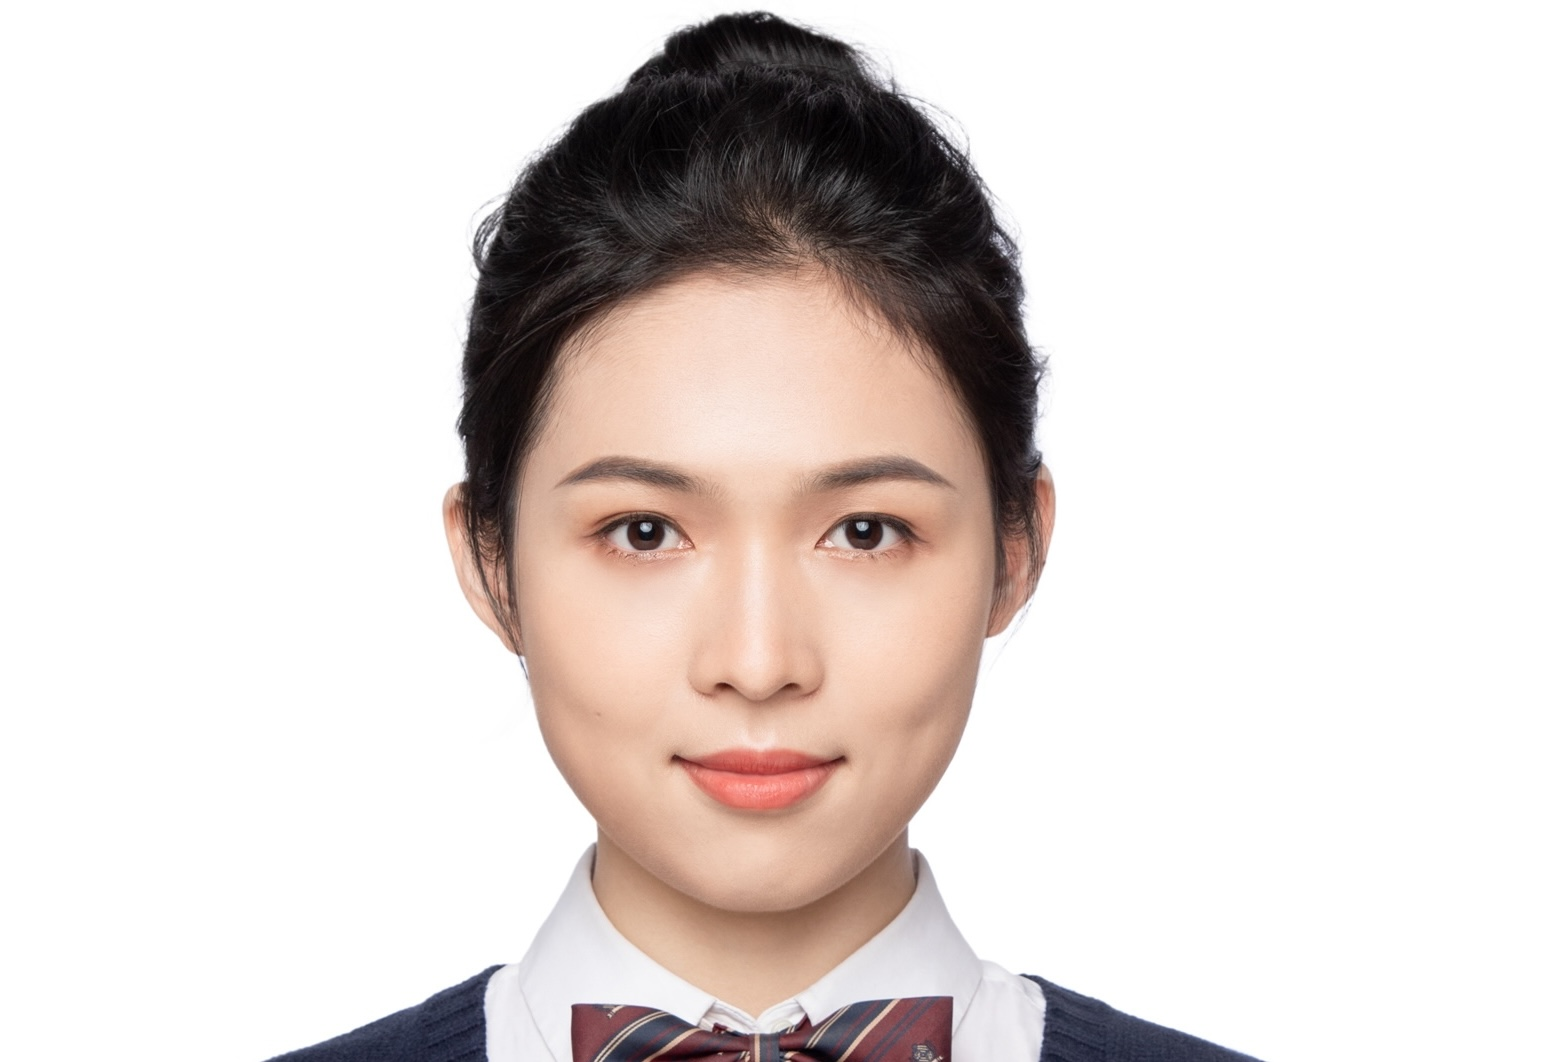
\includegraphics[width=\linewidth]{photo.jpg}
% \end{minipage}

\section{\faGraduationCap\ Education}
\datedsubsection{\textbf{Renmin University of China}, Beijing, China}{2022 -- Present}
\textit{PhD Candidate} in Artificial Intelligence (AI), { GPA }3.88/4.0
\begin{itemize}
  \item {Supervisor: }Prof. \href{https://weizhewei.com}{\it \underline{\textcolor{blue}{Zhewei Wei}}} at the \href{https://weizhewei.com/people}{\it \underline{\textcolor{blue}{ALGO Lab}}}
  \item {Research Interests: } LLM Agents, Recommendation, Graph Neural Networks
  \item {Awards: } {\bf China National Scholarship}
\end{itemize}
\datedsubsection{\textbf{Beijing University of Posts and Telecommunications}, Beijing, China}{2018 -- 2022}
\textit{B.S.} in Computer Science (CS), GPA 91.24/100, Rank 2.5\%
\begin{itemize}
  \item {\bf Awards: } Outstanding Graduate, First Prize Scholarship, Jiongpan Zhou Scholarship (Only one student in the school is selected each year), First Prize in NSCSCC 2020
\end{itemize}

\section{\faCogs\ Internships}
\datedsubsection{{\bf Alibaba: Tongyi Group}}{2025.05 -- 2026.05}
Research Intern | Mentors: \href{https://osier-yi.github.io/}{\textcolor{blue}{\underline{Liuyi Yao}}}, \href{https://xieyxclack.github.io/}{\textcolor{blue}{\underline{Yuexiang Xie}}}, \href{https://sites.google.com/site/yaliangli/}{\textcolor{blue}{\underline{Yaliang Li}}} \\
{\bf Open-source Contributions:}
\begin{itemize}
  \item \href{https://github.com/agentscope-ai/agentscope}{\textcolor{blue}{\underline{AgentScope}}}: Designed a hierarchical memory system for context and long-term memory management.
  % \begin{itemize}
  %   \item[\ding{182}] Automatic long-context processing: supports unbounded context windows via dynamic compression.
  %   \item[\ding{183}] Context offloading: persists non-critical content to the file system and retrieves on demand.
  %   \item[\ding{184}] Vector database integration: enables semantic retrieval and reasoning over long-term memory.
  %   \item[\ding{185}] Achieves 100\%+ relative gain in mean@3 on {BrowseComp-Plus} with Qwen3-max.
  % \end{itemize}
  \item \href{https://github.com/modelscope/trinity-rft}{\textcolor{blue}{\underline{Trinity-RFT}}}: Fixed bugs to resolve over-rollout inefficiency.
\end{itemize}
{\bf Research:} Context management for long-horizon tasks via end-to-end reinforcement learning
\begin{itemize}
  \item Trains an external LLM to manage the agent's context and learns agent-compatible strategies without retraining the agent itself.
  \item Substantially improves diverse agents on web search and deep research tasks, mitigating constraint forgetting, premature abandonment, and redundant exploration.
  \item Identifies the Fidelity--Reliability Trade-off and demonstrates that trained managers transfer most effectively across capability-similar agents.
\end{itemize}

\datedsubsection{{\bf Tencent: Hunyuan (Qingyun Talent Internship)}}{2026.06 -- Present}
Research Intern | Mentors: \href{https://p2333.github.io/}{\textcolor{blue}{\underline{Tianyu Pang}}}, \href{https://likaixin2000.github.io/}{\textcolor{blue}{\underline{Kaixin Li}}}\\
{\bf Research:} Long Video Generation Agent. [Ongoing]
\section{\faLeanpub\ Selected Publications}

\subsection{\bf Learning Agent-Compatible Context Management for Long-Horizon Tasks}
\role{{\textbf{Lu Yi},
 Runlin Lei,
 Liuyi Yao,
 Yuexiang Xie,
 Wenhao Zhang,
 Zhewei Wei,
 Yaliang Li,
 Jian-Yun Nie, et al.} [\href{http://arxiv.org/abs/2605.30785}{\textcolor{blue}{\underline{PDF}}}]}
\par\noindent An adaptive context management framework that trains an external LLM to manage the context of a frozen agent through flexible modification actions and end-to-end reinforcement learning.
\subsection{\bf Future Link Prediction Without Memory or Aggregation}
\role{{\textbf{Lu Yi}, Runlin Lei, Fengran Mo, Yanping Zheng, Zhewei Wei, Yuhang Ye.} NeurIPS 2025. [\href{https://arxiv.org/abs/2505.19408}{\textcolor{blue}{\underline{PDF}}}]}
\par\noindent A simple yet effective method for future link prediction that excels in real-world recommendation.

\subsection{\bf TGB-Seq Benchmark: Challenging Temporal GNNs with Complex Sequential Dynamics}
\role{ {\textbf{Lu Yi}}, Jie Peng, Yanping Zheng, Fengran Mo, Zhewei Wei, et al. ICLR 2025. [\href{https://openreview.net/pdf?id=8e2LirwiJT}{\textcolor{blue}{\underline{PDF}}}] [\href{https://tgb-seq.github.io/}{\textcolor{blue}{\underline{Website}}}]}
\par\noindent A new benchmark for future link prediction involving complex sequential dynamics.

\subsection{{\bf Scalable and Certifiable Graph Unlearning: Overcoming the Approximation Error Barrier} }
\role{ {\textbf{Lu Yi}}, Zhewei Wei. ICLR 2025 (\textbf{Spotlight}). [\href{https://openreview.net/pdf?id=pPyJyeLriR}{\textcolor{blue}{\underline{PDF}}}]}
\par\noindent The first approach to scale certified graph unlearning to billion-edge graphs.

\subsection{\bf Optimal Dynamic Subset Sampling: Theory and Applications}
\role{{\textbf{Lu Yi}}, Hanzhi Wang, Zhewei Wei. KDD 2023 (\textbf{Oral}). [\href{https://dl.acm.org/doi/10.1145/3580305.3599458}{\textcolor{blue}{\underline{PDF}}}]}
\par\noindent The first dynamic subset sampling algorithm with optimal sampling and update time complexity.

\subsection{\bf Random-Walk Probability Estimation on Dynamic Weighted Graphs}
\role{{Hanzhi Wang*, {\textbf{Lu Yi}}*, Zhewei Wei.} Journal of Computer Research and Development (J-CRAD) 2024.\\ Invited \textbf{oral} presentation at China Conference on Data Mining (CCDM) 2024. [\href{https://crad.ict.ac.cn/article/doi/10.7544/issn1000-1239.202440148}{\textcolor{blue}{\underline{PDF}}}]}
\par\noindent A random walk framework by coin-flip sampling to estimate $L$-hop random-walk probabilities.

\subsection{\bf Robustness in Text-Attributed Graph Learning: Insights, Trade-offs, and New Defenses}
\role{Runlin Lei, {\textbf{Lu Yi}}, Mingguo He, Pengyu Qiu, Zhewei Wei, et al. ICLR 2026. [\href{https://openreview.net/pdf?id=CEJl0gN2gj}{\textcolor{blue}{\underline{PDF}}}]}
\par\noindent Systematic evaluation of TAG model robustness against adversarial attacks.

\subsection{\bf A survey of dynamic graph neural networks}
\role{Yanping Zheng, {\textbf{Lu Yi}}, Zhewei Wei. Frontiers of Computer Science 2024. [\href{https://journal.hep.com.cn/fcs/EN/10.7544/issn1000-1239.202440148}{\textcolor{blue}{\underline{PDF}}}]}
\par\noindent A comprehensive review of dynamic graph neural networks.

\section{\faHeartO\ Personal AI Tools}
\datedsubsection{{\bf CCManager: Multi-Device Task Manager for Claude Code}} {\it[\href{https://github.com/luyi256/CCManager}{\textcolor{blue}{\underline{CODE}}}]}
\begin{itemize}
  \item Orchestrate Claude Code tasks across multiple devices via mobile-friendly Web UI with voice input.
  \item Security-first design: Docker sandbox isolation, Git worktree for safe parallel development.
  \item Real-time streaming output, session resume, and plan-mode review for human-in-the-loop control.
\end{itemize}

\end{document}
